\documentclass[a4paper, 12pt]{article}

\usepackage[italian]{babel}
\usepackage{tikz}
\usepackage{xcolor}
\usepackage{graphicx}
\usepackage{hyperref}
\usepackage{imakeidx}
\usepackage{caption}
\usepackage{fancyhdr}
\usepackage{tabularx}
\usepackage{ragged2e}

%--------------------VARIABILI--------------------
\def\logo{../Immagini/logo.jpeg}
\def\ultima-versione{v0.2}
\def\titolo{Norme di Progetto }
%------------------------------------------------

\usetikzlibrary{calc}
\definecolor{fp-blue}{HTML}{2885c8}
\definecolor{fp-red}{HTML}{ea5f64}
\makeindex[title=Indice]
\hypersetup{hidelinks}

\pagestyle{fancy}
\fancyhead[L]{}
\setlength{\headheight}{15pt}
\fancyhead[R]{\titolo - \ultima-versione}

\renewcommand{\familydefault}{\sfdefault}
\newcommand{\glossario}[1]{\fontfamily{lmr}\selectfont{\textit{#1\textsubscript{\small G}}}}

%--------------------INFORMAZIONI PRIMA PAGINA-------------------- 
\title{\Huge \textbf{\titolo}}
\author{\Large{Alt} \raisebox{0.3ex}{\normalsize  +} \Large{F4}}
\date{\today}
%----------------------------------------------------------------

\begin{document}

\begin{titlepage}      
    \maketitle
    \thispagestyle{empty}  

    \begin{tikzpicture}[remember picture, overlay]
        \fill[fp-blue] 
        ($(current page.south west) + (0, 10)$) 
        -- ($(current page.center) + (0, -8)$)
        -- ($(current page.center) + (0, -15)$)
        -- (current page.south west);

        \fill[fp-red]
        ($(current page.south east) + (0, 10)$) 
        -- ($(current page.center) + (0, -8)$)
        -- ($(current page.center) + (0, -15)$)
        -- (current page.south east);

        \clip ($(current page.center) + (0, -8)$) circle (1cm) node 
        {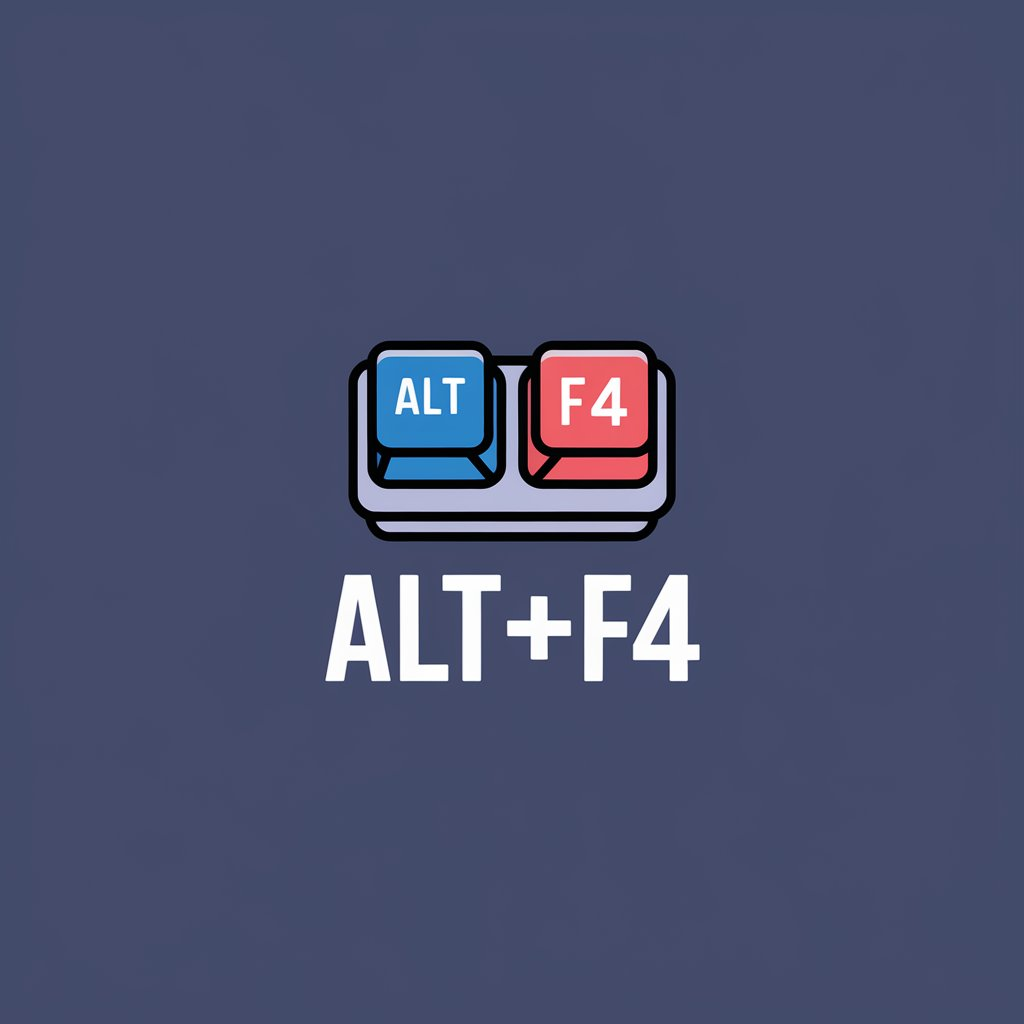
\includegraphics[width=.25\textwidth]{\logo}};
        
    \end{tikzpicture}    
\end{titlepage}

\tableofcontents

\newpage

\begin{table}[!h]
    \centering
    \caption*{\textbf{\Large Registro Modifiche}}
    {\renewcommand{\arraystretch}{2}
    \begin{tabularx}{\textwidth}{| X | X | X | X |}
        \hline
            \textbf{\large Versione} & 
            \textbf{\large Data} & 
            \textbf{\large Autore/i} & 
            \textbf{\large Descrizione} \\ 
        \hline \hline
            v0.1 & 
            25/10/2024 & 
            Enrico Bianchi & 
            Stesura documento \\
        \hline 
        \ultima-versione & 
            26/10/2024 & 
            Pedro Leoni & 
            Modifica sezioni "template" e "organizzazione repository"  \\
        \hline 
    \end{tabularx}}
\end{table}

\newpage

    \section{Introduzione}
    Il seguente documento "Norme di Progetto" ha lo scopo di definire strumenti di lavoro e pratiche comuni adottati dal team per garantire una metodologia di lavoro efficiente ed efficace.
    Questo documento verrà quindi utilizzato come guida dal team in caso vi siano dubbi su come lavorare.

    \section{Canali di comunicazione}
    
    \subsection{Comunicazioni interne}
    Il gruppo ha stabilito di utilizzare Telegram come chat di gruppo per le discussioni rapide e di usare Discord per le riunioni. 
    Il motivo di questa scelta è di mantenere una comunicazione fluida e immediata tra i membri del team, facilitando il coordinamento e la condivisione di idee.
    
    \subsection{Comunicazioni esterne}
    Si è deciso di utilizzare Gmail come servizio di posta elettronica per comunicare sia con il proponente che con il docente. 
    Per le riunioni con il proponente, si opterà per Zoom, che offre funzionalità avanzate per le conferenze online.

    \section{Documentazione}
    
    \subsection{Stesura documenti}
    Per la stesura della documentazione il gruppo ha deciso di utilizzare Google Docs per una prima fase di scrittura veloce e collaborativa, poiché consente di lavorare in modo immediato e intuitivo, inoltre permette al team di annotare idee in tempo reale durante le riunioni. Una volta definita l’idea e il contenuto del documento, si procederà alla redazione definitiva utilizzando LaTeX. La scelta di LaTeX è motivata non solo dalla necessità di gestire al meglio il versionamento, cosa non possibile con Google Docs, ma anche per acquisire competenze su uno strumento altamente rilevante per il percorso accademico.
    
    \subsubsection{Template}
    E’ stato deciso di utilizzare un template per la stesura dei documenti di progetto che: importa i pacchetti necessari, definisce la pagina iniziale, definisce l’indice dei contenuti e definisce il registro delle modifiche. 
    Inoltre il template mostra l’applicazione di un insieme di marcatori di uso comune.
    Per la creazione di un nuovo documento il componente del team deve:
    \begin{itemize}
        \item Copiare il contenuto del template nel nuovo file sorgente LaTeX.
        \item Cambiare il valore delle variabili chiamate titolo, ultima-versione e logo.
        \item Eliminare gli esempi d'uso dei marcatori LaTex.
    \end{itemize}
    Notare che il componente non deve modificare le informazioni della prima pagina ma limitarsi a cambiare i valori delle variabili.

    \subsection{Versione documenti}
    Per indicare le diverse versioni dei documenti è stato deciso di utilizzare uno schema di versionamento avente forma vX.Y con X e Y numeri naturali dove il primo indica una versione principale mentre il secondo indica una versione secondaria.
    La versione principale rappresenta un cambiamento significativo nel documento che produce una versione finale o stabile.
    Quando viene incrementata la versione principale la versione secondaria viene azzerata.
    La versione secondaria rappresenta un cambiamento minore sul contenuto del documento come l’aggiunta o la modifica di una parte del suo contenuto.
    Una volta definita una nuova versione di un documento esso non può essere modificato senza generare una nuova versione.

    \subsection{Organizzazione repository}
    Per la gestione e la condivisione dei documenti si è deciso di utilizzare GitHub, che fornisce inoltre un sistema di Issue Tracking System intuitivo, che consente di segnalare, discutere e risolvere i problemi in modo collaborativo.
    Il gruppo si è quindi dotato di un organization account che si può trovare al link \url{https://github.com/ALT-F4-eng}.
    Successivamente si è quindi creato il repository pubblico per la documentazione, \url{https://github.com/ALT-F4-eng/Documentazione}, che conterrà i sorgenti LaTeX:
    \begin{itemize}
        \item \textbf{Verbali interni}: documentano le riunioni interne del gruppo.
        \item \textbf{Verbali esterni}: documentano riunioni con le aziende proponenti.
        \item \textbf{Documenti di progetto}: glossario e norme di progetto.
    \end{itemize}
    I verbali interni verranno messi nella cartella "VerbaliInterni" e verranno denominati seguendo lo schema "data\_versione".
    I verbali esterni verranno messi nella cartella "VerbaliEsterni" e verranno denominati seguendo lo schema "data\_versione". 
    I documenti di progetto verranno messi nella cartella "DocumentiInterni" e verranno denominati aggiungendo in coda la loro verisone.
    
    \subsection{Workflow}
    Per la gestione dei branch del repository è stato deciso di utilizzare il modello di branching \href{https://www.atlassian.com/it/git/tutorials/comparing-workflows/gitflow-workflow}{GitFlow}.
    In particolare per la documentazione è stato deciso di usare:
    \begin{itemize}
        \item I rami \textbf{/feature/*} per la definizione di nuove versioni minori.
        \item Il ramo \textbf{develop} per registrare le versioni minori.
        Prima la versione minore deve essere revisionata da un componente del team diverso dal creatore mediante una pull request.
        In particolare prima di chiudere la pull request  il revisionatore deve eseguire un commit sul ramo da fondere dove aggiorna il registro delle modifiche.
        L’accettazione di una versione minore produce quindi un’altra versione minore dato che modifica il documento stesso.
        \item Il ramo \textbf{main} viene usato per pubblicare le versioni dei documento all’esterno del team di lavoro.
    \end{itemize}

\end{document}